\chapter{Force Torque Sensor Compensation}
\label{chapter:ft-sensor-correction}

% ADD: Dar introdução ao capítulo
\par In this chapter... (\textbf{dar a outline do capítulo})

\section{Force Torque Sensor Correction}

\par To achieve the tasks that require physical contact between the human and the cobot, the UR10e built-in \ac{ft} sensor, located at its \ac{eef} will be extensively used. Its technical specifications can be found in \autoref{tbl:ur10e-specs}. There are two ways of interfacing with the sensor, both of them managed by the URControl controller. One of them is through URScript commands, with \textit{get\_tcp\_force()} used for obtaining the \ac{ft} values at the \acs{tcpr}, and \textit{zero\_ftsensor()} that zeroes the \ac{ft} measurement by subtracting the current measurement from the subsequent. The other, is using the \ac{ur} \ac{ros} Driver which publishes the \ac{ft} measurement in the \textbackslash\textit{wrench} topic at 500Hz, and exposes the \textbackslash\textit{zero\_ftsensor} service. Relevant to this matter, the Polyscope interface has a configuration parameter used to describe the weight coupled to the \acs{tcpr}, called Payload. It is composed of mass, in Kg, and \ac{cog}, in cartesian coordinates, and their effect on the \ac{ft} measurement will be later demonstrated in \autoref{ssec:ft_internal_comp}.

\subsection{Noise Filtering}

% LER: Signal Processing and Application of Six-axis Force/Torque Sensor Integrated in Humanoid Robot Foot

\par As seen in \autoref{tbl:ur10e-specs}, the \ac{ur10e} \ac{ft} sensor has a reported resolution of 2 N on force, and 0.02 Nm on torque measurements. The 2 graphs on the left of \autoref{fig:ft_sensor_filter} demonstrate that this fact is due to the noise generated by the hardware of the sensor. 

\begin{equation}
    \mathbf{W_{fil}} = (1-\alpha)W_n + \alpha \left(\frac{W_n + W_{n-1}}{2}\right)
    \label{eq:wrench_filter}
\end{equation}

% Moving Average Filter
% https://maker.pro/arduino/tutorial/how-to-clean-up-noisy-sensor-data-with-a-moving-average-filter#:~:text=What%20is%20a%20Moving%20Average,frequency%20information%20from%20the%20output.
% Low Pass Filter
% https://dobrian.github.io/cmp/topics/filters/lowpassfilter.html#:~:text=Introduction,lower%20frequencies%20to%20pass%20through.&text=In%20a%20digital%20signal%20received,contain%20occasional%20spurious%20incorrect%20values.

\par The chosen way of dealing with this noise is to apply a \ac{lpf} to the raw measurements. \autoref{eq:wrench_filter} defines a 2\textsuperscript{th} order \ac{fir} filter with an average component added to it. Other types of \acp{lpf} were also considered, such as a \ac{maf} but the results were not satisfactory.

\par A \ac{ros} node with the purpose of filtering the raw measurements was developed. It subscribes to the \textbackslash \textit{wrench} topic, filters each value with \autoref{eq:wrench_filter} and publishes them in the \textbackslash \textit{wrench\_filtered} topic. The $\alpha$ parameter can be changed in real-time using the \ac{ros} dynamic reconfigure tool. Tests showed that an $\alpha = 0.2 $ was satisfactory for noise reduction without major delay impact on the measurements. Results of this filtering technique can be observed in the graphs on the right of \autoref{fig:ft_sensor_filter}.

\begin{figure}[h]
    \centering
    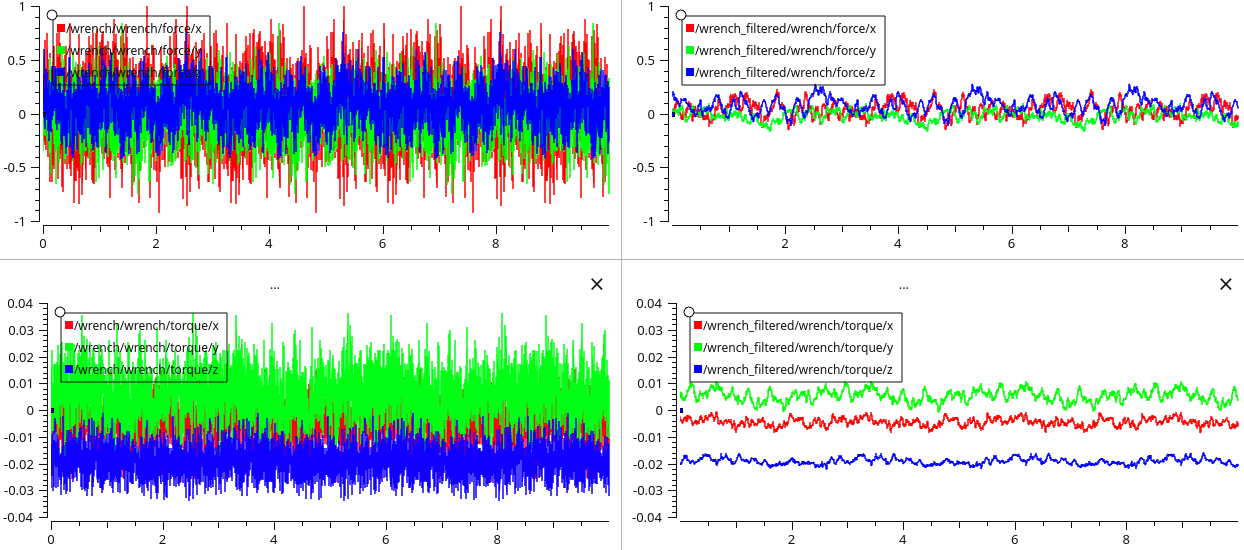
\includegraphics[width=0.9\linewidth]{figs/chp3/ft_sensor_filter.png}
    \caption{Comparison of raw and noise filtered \ac{ft} measurements}
    \label{fig:ft_sensor_filter}
\end{figure}


\subsection{Force Torque Sensor Observed Behavior}

\par Further experiments with the \ac{ft} sensor measurements showed a couple of unexpected behaviors outline in the following subsections.

\subsubsection{Wrist3 Joint Positional Variation}

\par The measurements of the \ac{ft} sensor present variations relative to the position of the Wrist3 joint. \autoref{fig:w3_problem} shows a simple real time test where the \ac{eef} is fixed in a random pose, and the Wrist3 joint is rotated from $-2\pi$ to $2\pi$. The \ac{ft} measurements present clear variations that can reach 8N of difference from the correct value, which should be close to 0N the entire test since the \ac{eef} has no tool or weight coupled to it. Changing the pose of the \ac{eef} presented the same results. 

\begin{figure}[h]
    \centering
    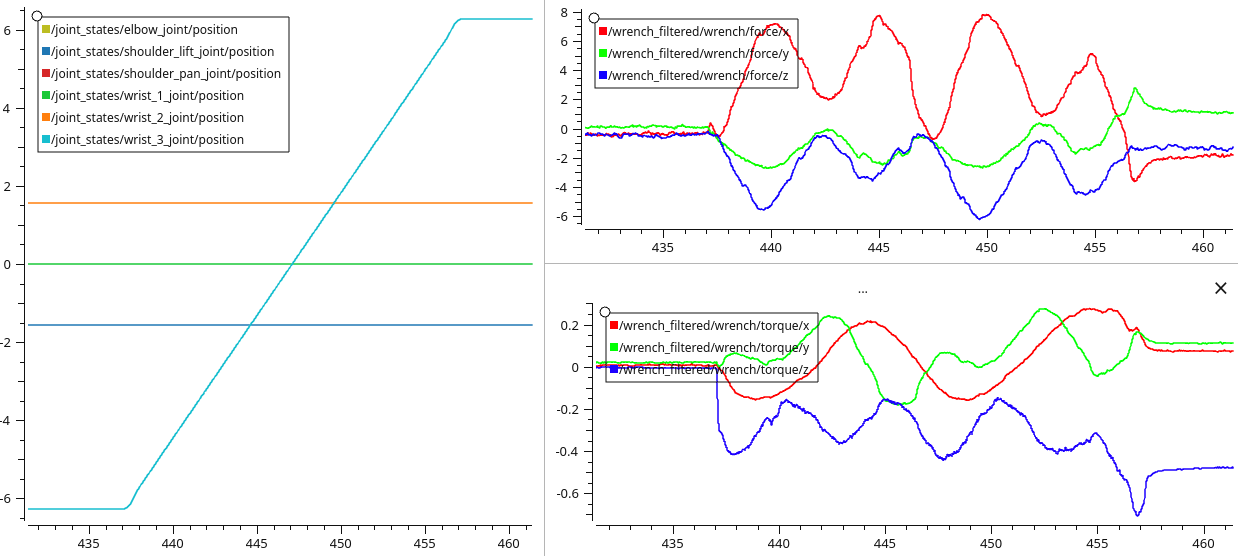
\includegraphics[width=0.9\linewidth]{figs/chp3/wrist_3_problem.png}
    \caption{Variation on \ac{ft} relative to the position of the Wrist3 joint}
    \label{fig:w3_problem}
\end{figure}

\par This presents a problem for the accuracy of the \ac{hg} and object manipulation tasks since an error of 8N is significant. \autoref{ssec:w3_solution} demonstrates the proposed solution for this problem.

\subsubsection{Temporal Drift}

\par When the robot is left still for long periods of time, the values of \ac{ft} can change linearly as much as $0.2\si{N}/\si{min}$. It might not seem a significant value, but if an \ac{hg} task were to be activated, by letting the cobot stand still for a couple of minutes, it would start moving on its owm. A recording of \ac{ft} values over a period of 10 minutes, with a step of 200ms is shown in \autoref{fig:ft_sensor_drift}. 

\begin{figure}[h]
    \centering
    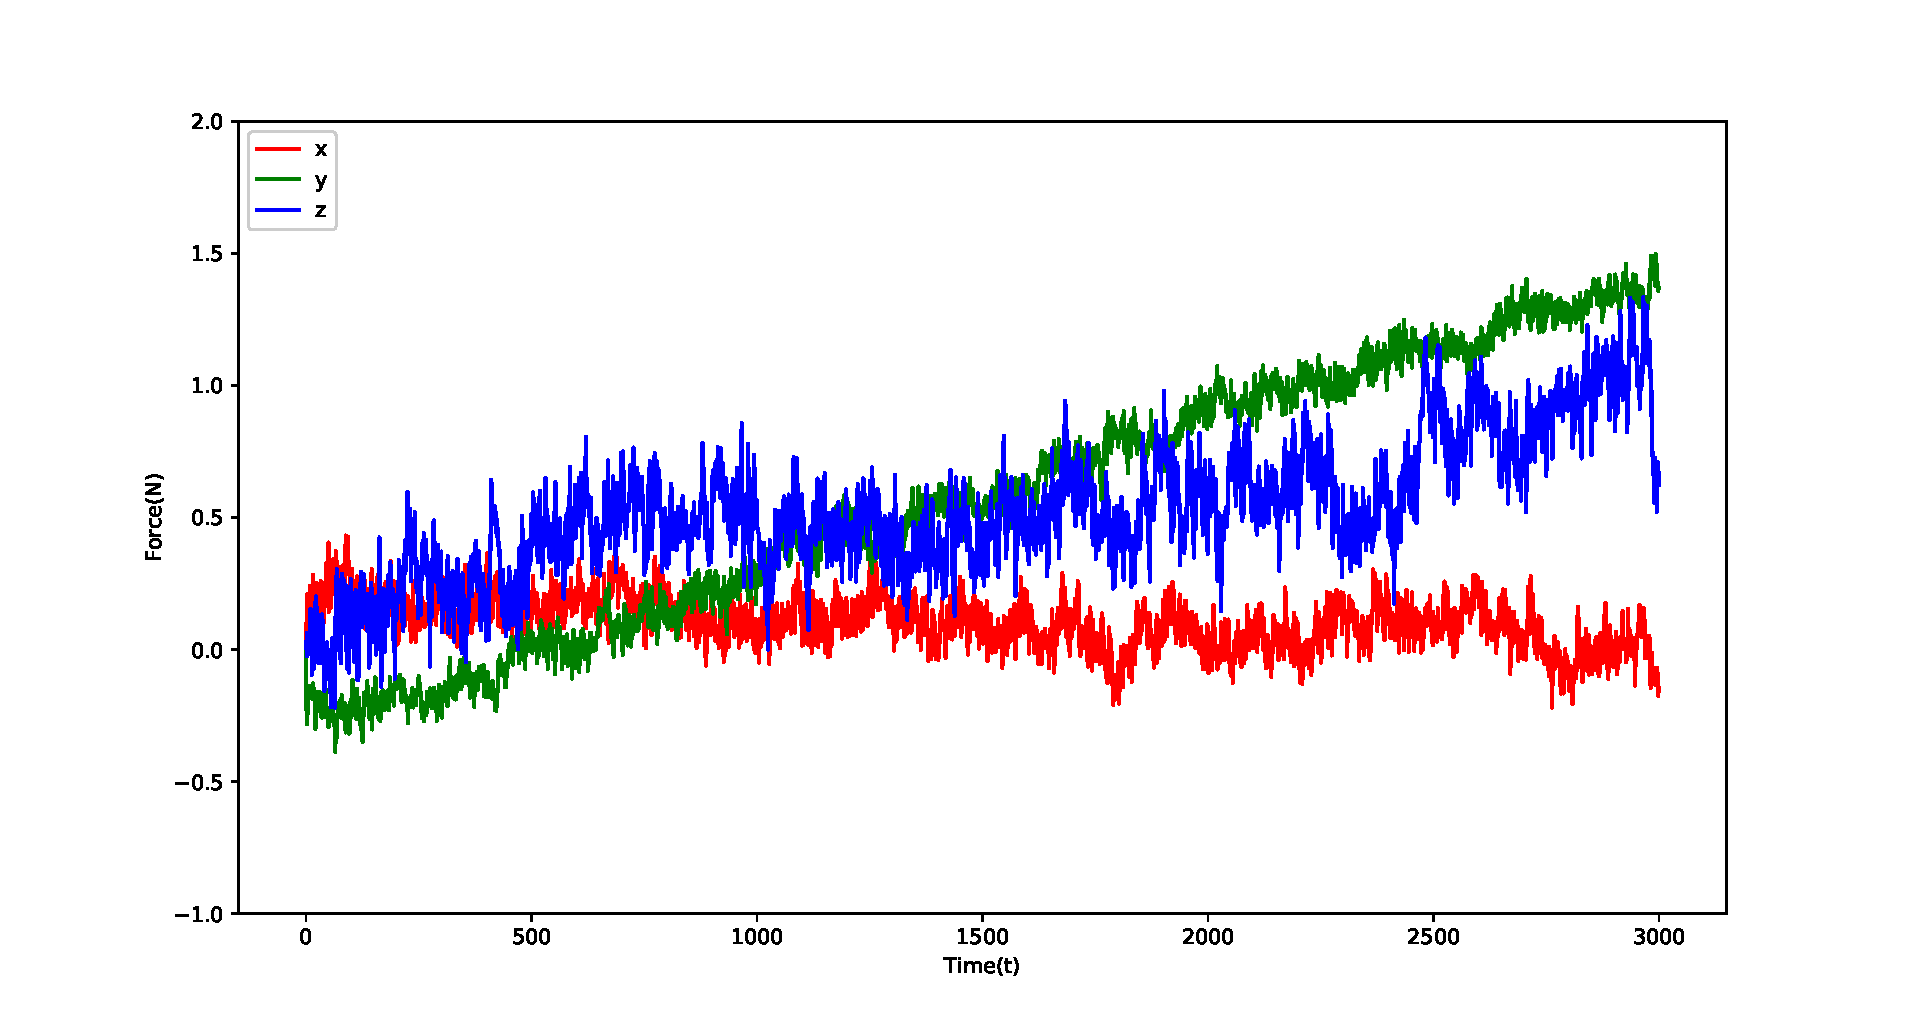
\includegraphics[width=\linewidth]{figs/chp3/ft_sensor_drift.pdf}
    \caption{Variation of \ac{ft} relative to time}
    \label{fig:ft_sensor_drift}
\end{figure}

\par Using the zero\_ftsensor in a recurring, timely manner would fix this problem but raise the issue on when to do so, since it might also erase important \ac{ft} measurements needed for the executing task.

\subsubsection{Variations caused by \ac{ft} applied}

\par Applying high amounts of external \ac{ft} to the sensor, will result in a variation on the measurements after its removed. This behavior can be seen in \autoref{fig:ft_sensor_pushes} where every time there is a strong interaction with the \ac{eef}, the subsequent values of \ac{ft} present variations as high as 3N and 0.3Nm.

\begin{figure}[h]
    \centering
    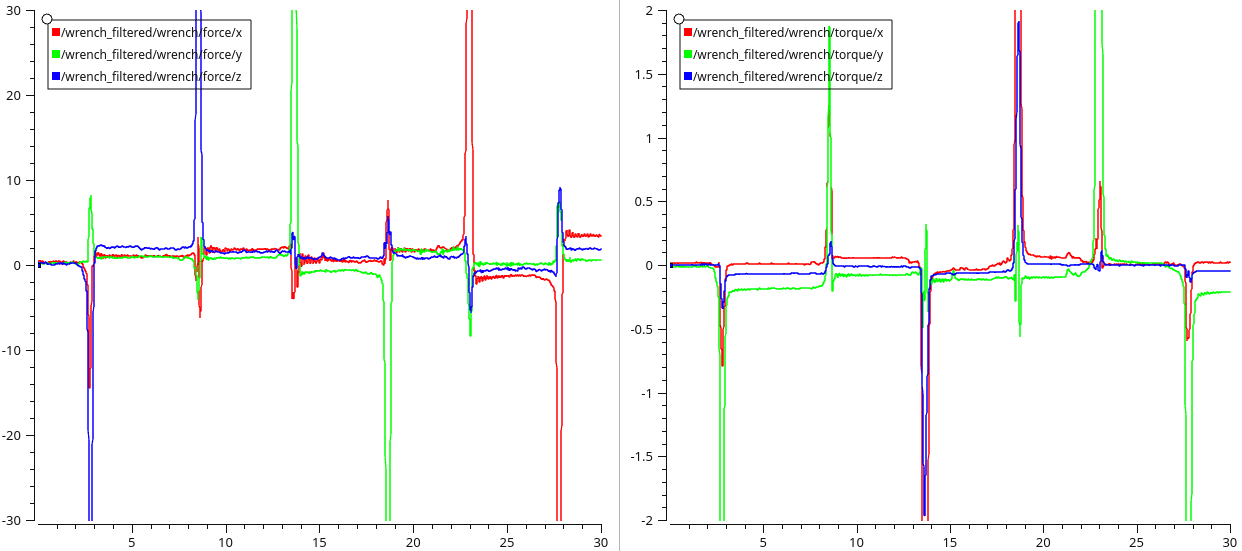
\includegraphics[width=0.9\linewidth]{figs/chp3/ft_sensor_pushes.png}
    \caption{Variation in \ac{ft} relative to interaction with the \ac{eef}}
    \label{fig:ft_sensor_pushes}
\end{figure}

\par Similar to the previous problem, this measurements are wrongly introduced in the system, since the \ac{ft} felt by the sensor should not suffer alterations due to momentarily external interaction with the \ac{eef}.

\subsubsection{Special case of the Z-Axis}

\par Upon coupling a gripper tool to the \ac{eef} of the robot, it was clear that the force applied by screwing the mounting plate onto the \ac{eef} had effects on the values of force reported on the Z-Axis. The mounting plate in question has 4 screws, and even making sure they were evenly tightened, the stronger the tightening, the higher the force measurement on the Z-Axis.

\par Measurements of torque in the Z-Axis present momentary fixed variations depending on the amount of movement and direction of the Wrist3 joint. These variations can be seen in any of the live recording tests (\autoref{fig:w3_problem}, \autoref{fig:w3_result}, \autoref{fig:ft_theory_result}) but in practicality are irrelevant since they only occur when the robot is moving autonomously, not when the user is applying force to the \ac{eef}.

\subsection{Proposed Solution}
\label{ssec:w3_solution}

\par Regarding the variation of \ac{ft} relative to the Wrist3 joint position, tests were made to prove that the pattern of variation of the measurements was independent of the \ac{eef} orientation, therefore not caused by gravitational forces. The test in question consists on the rotation of the Wrist3 joint from \ang{-360} to \ang{360} in steps of \ang{1}. Each step, the average values of \ac{ft} in a time period of 0.1ms are calculated and saved. The result of the test is a matrix with shape [720, 2, 3], which means 720 values of \ac{ft} in the 3 cartesian axis. The test was performed in each of the 5 positions described in \autoref{fig:eef_5_position}, and its internal behavior can be seen in \autoref{code:w3_test}.

\begin{figure}[h]
    \centering
    \begin{subfigure}{.195\linewidth}
      \centering
      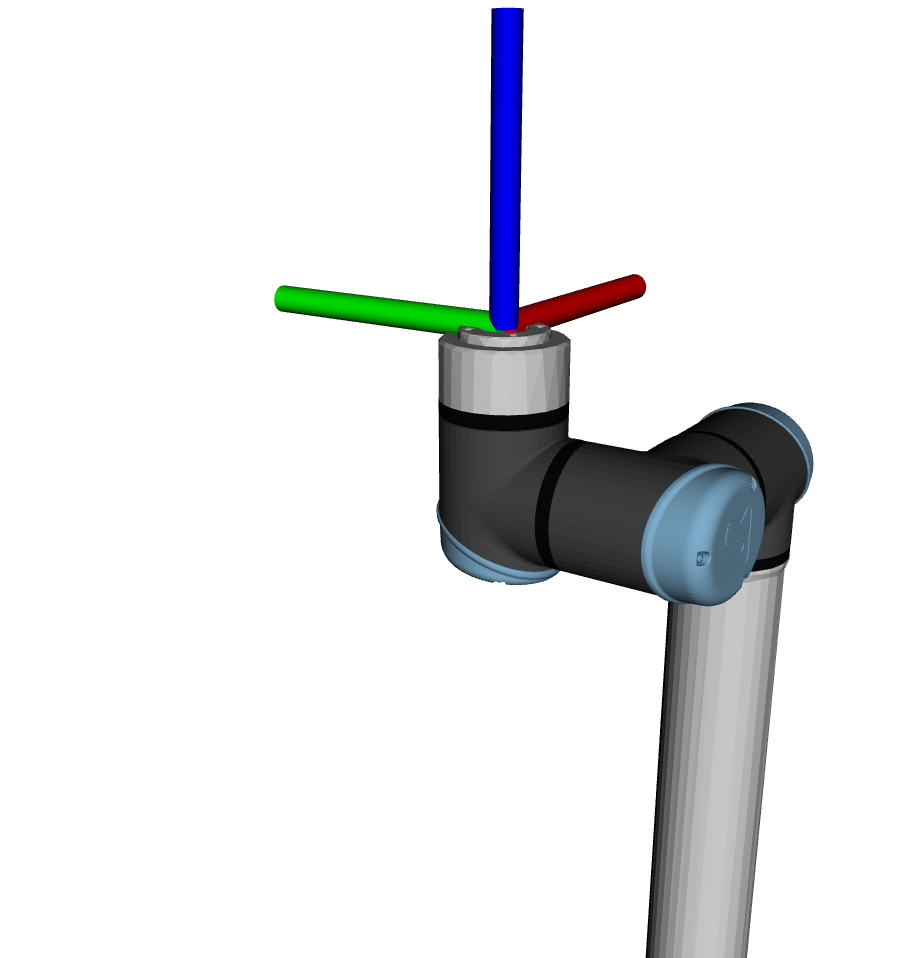
\includegraphics[width=\linewidth]{figs/chp3/P1.png}
      \label{fig:eef_p1}
    \end{subfigure}%
    \begin{subfigure}{.195\linewidth}
      \centering
      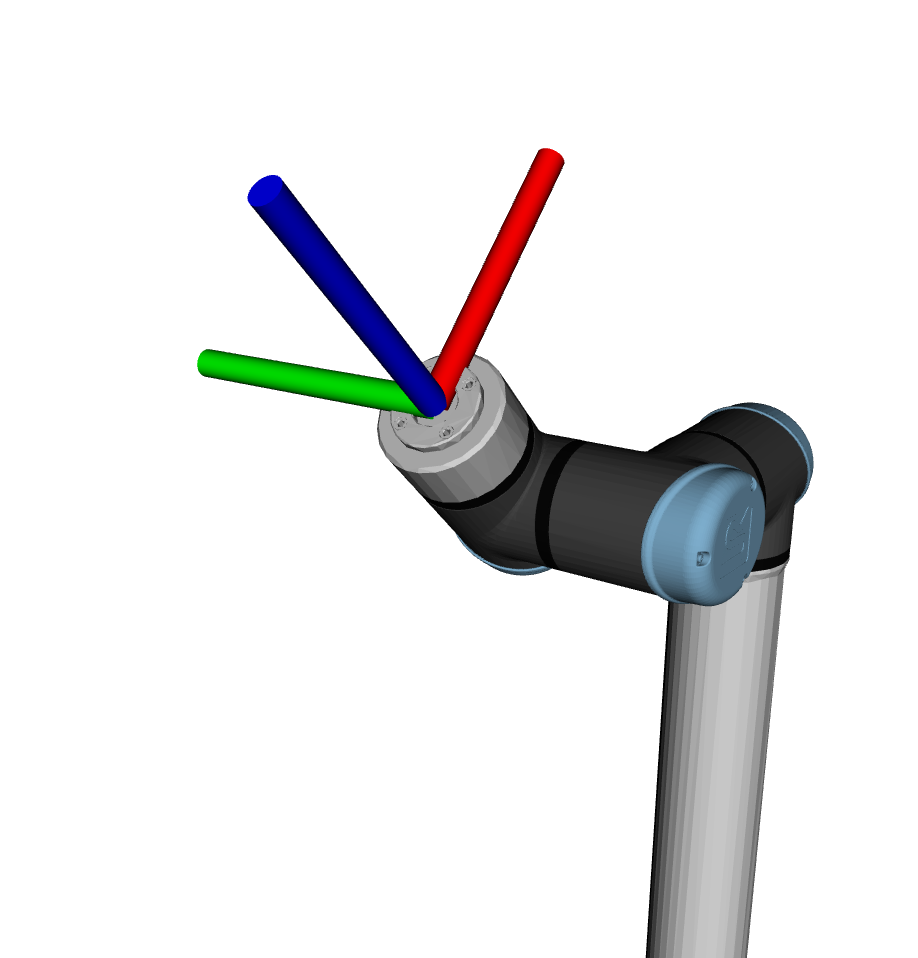
\includegraphics[width=\linewidth]{figs/chp3/P2.png}
      \label{fig:eef_p2}
    \end{subfigure}
    \begin{subfigure}{.195\linewidth}
        \centering
        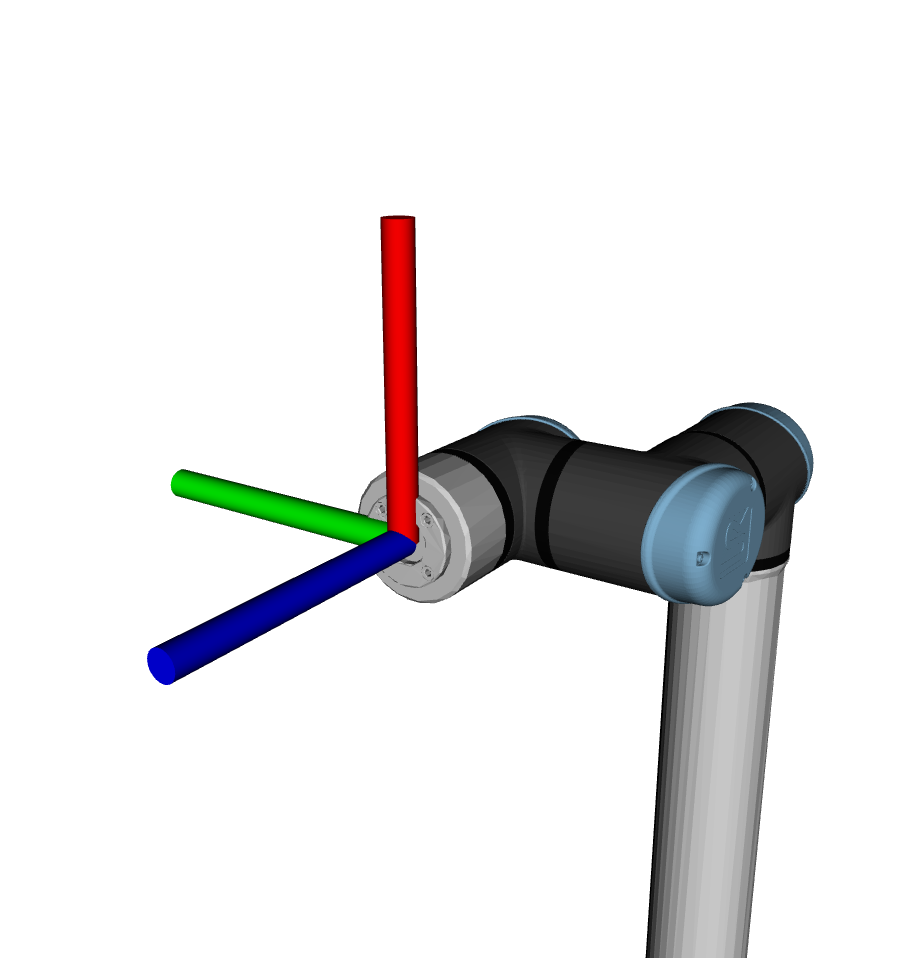
\includegraphics[width=\linewidth]{figs/chp3/P3.png}
        \label{fig:eef_p3}
    \end{subfigure}
    \begin{subfigure}{.195\linewidth}
        \centering
        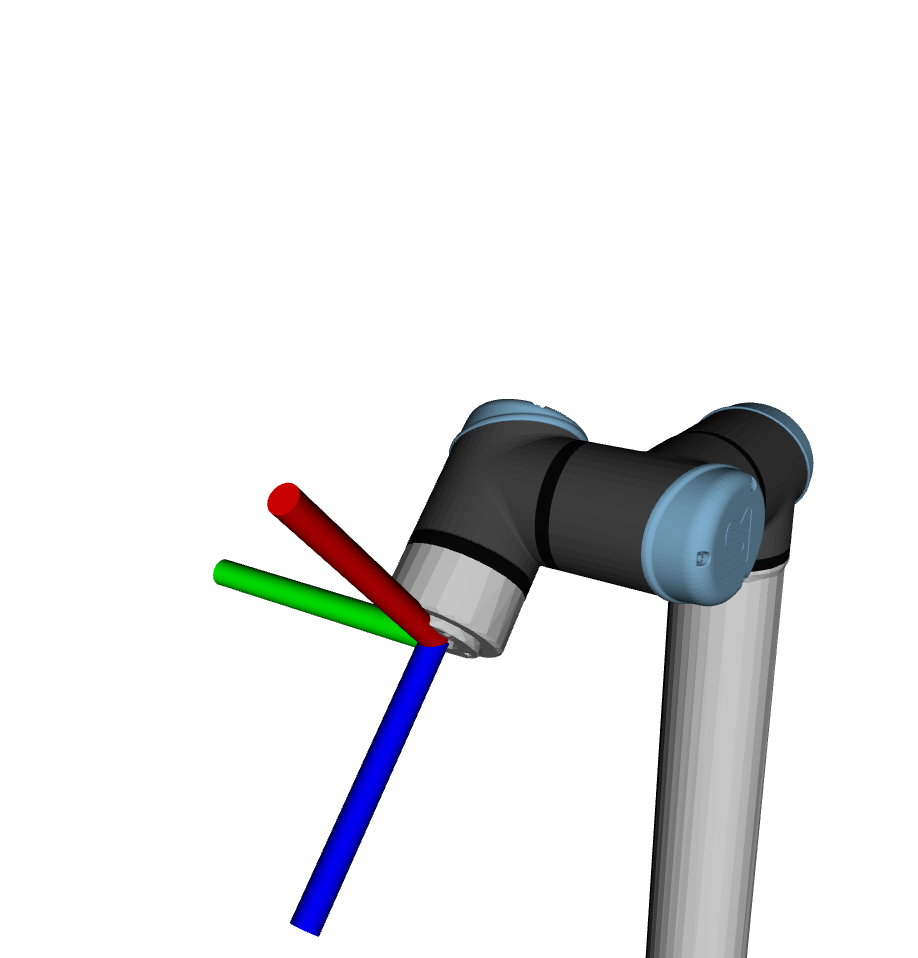
\includegraphics[width=\linewidth]{figs/chp3/P4.png}
        \label{fig:eef_p4}
    \end{subfigure}
    \begin{subfigure}{.195\linewidth}
        \centering
        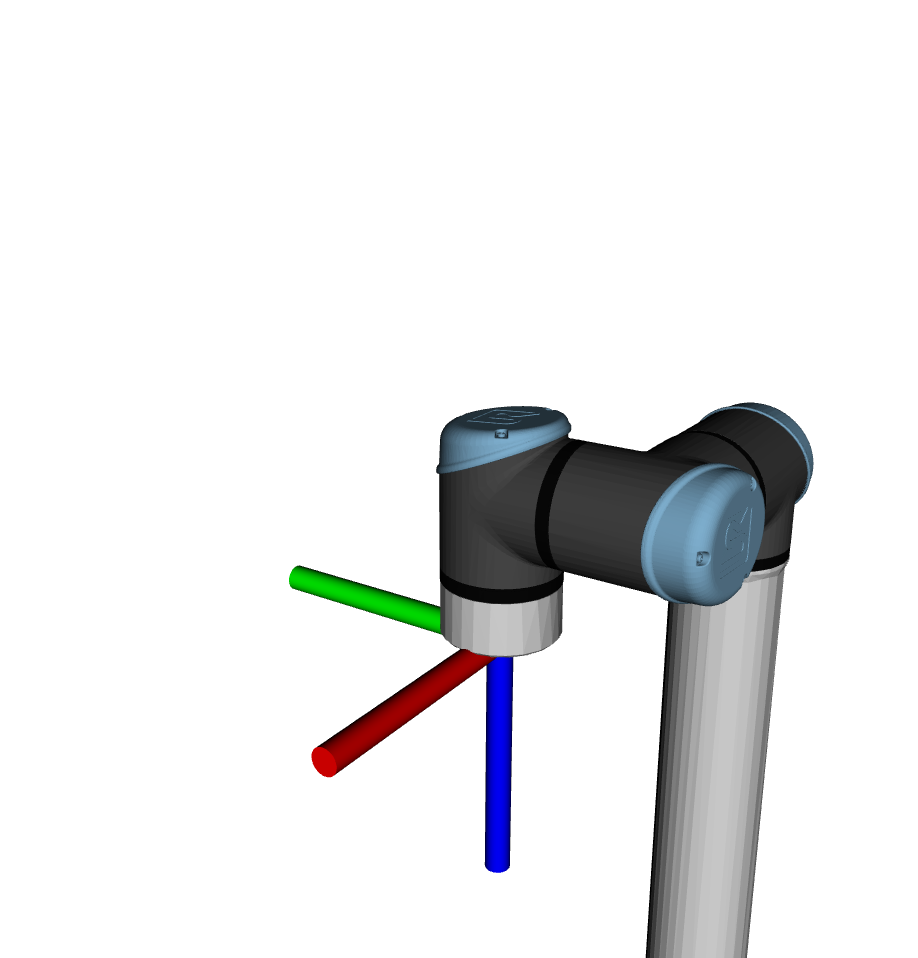
\includegraphics[width=\linewidth]{figs/chp3/P5.png}
        \label{fig:eef_p5}
    \end{subfigure}
    \caption{5 different \ac{eef} testing poses}
    \label{fig:eef_5_position}
\end{figure}

\begin{listing}[h]
    \centering
    \begin{minted}{python}

    wrench = Subscriber("\wrench", size=25)
    
    for pose in poses:
        ur10e.movePose(pose)
        ur10e.zero_ftsensor()
        test = Matrix(720, 2, 3)

        for position in range(-360, 360):
            ur10e.moveWrist3(position)
            sample = wrench.getAverage()
            test.append(sample.force, sample.torque)
        
        saveFile(test)   
    
    \end{minted}
\caption{Recording of \ac{ft} measurements in different poses}
\label{code:w3_test}
\end{listing}

\par The final test results can be seen in \autoref{fig:ft_sensor_test_5}. As predicted, the variation of \ac{ft} only has relation to the position of the Wrist3 joint. Furthermore, the standard deviation of the results is very low, meaning an accurate solution based on the average values recorded can be implemented.

\begin{figure}[h]
    \centering
    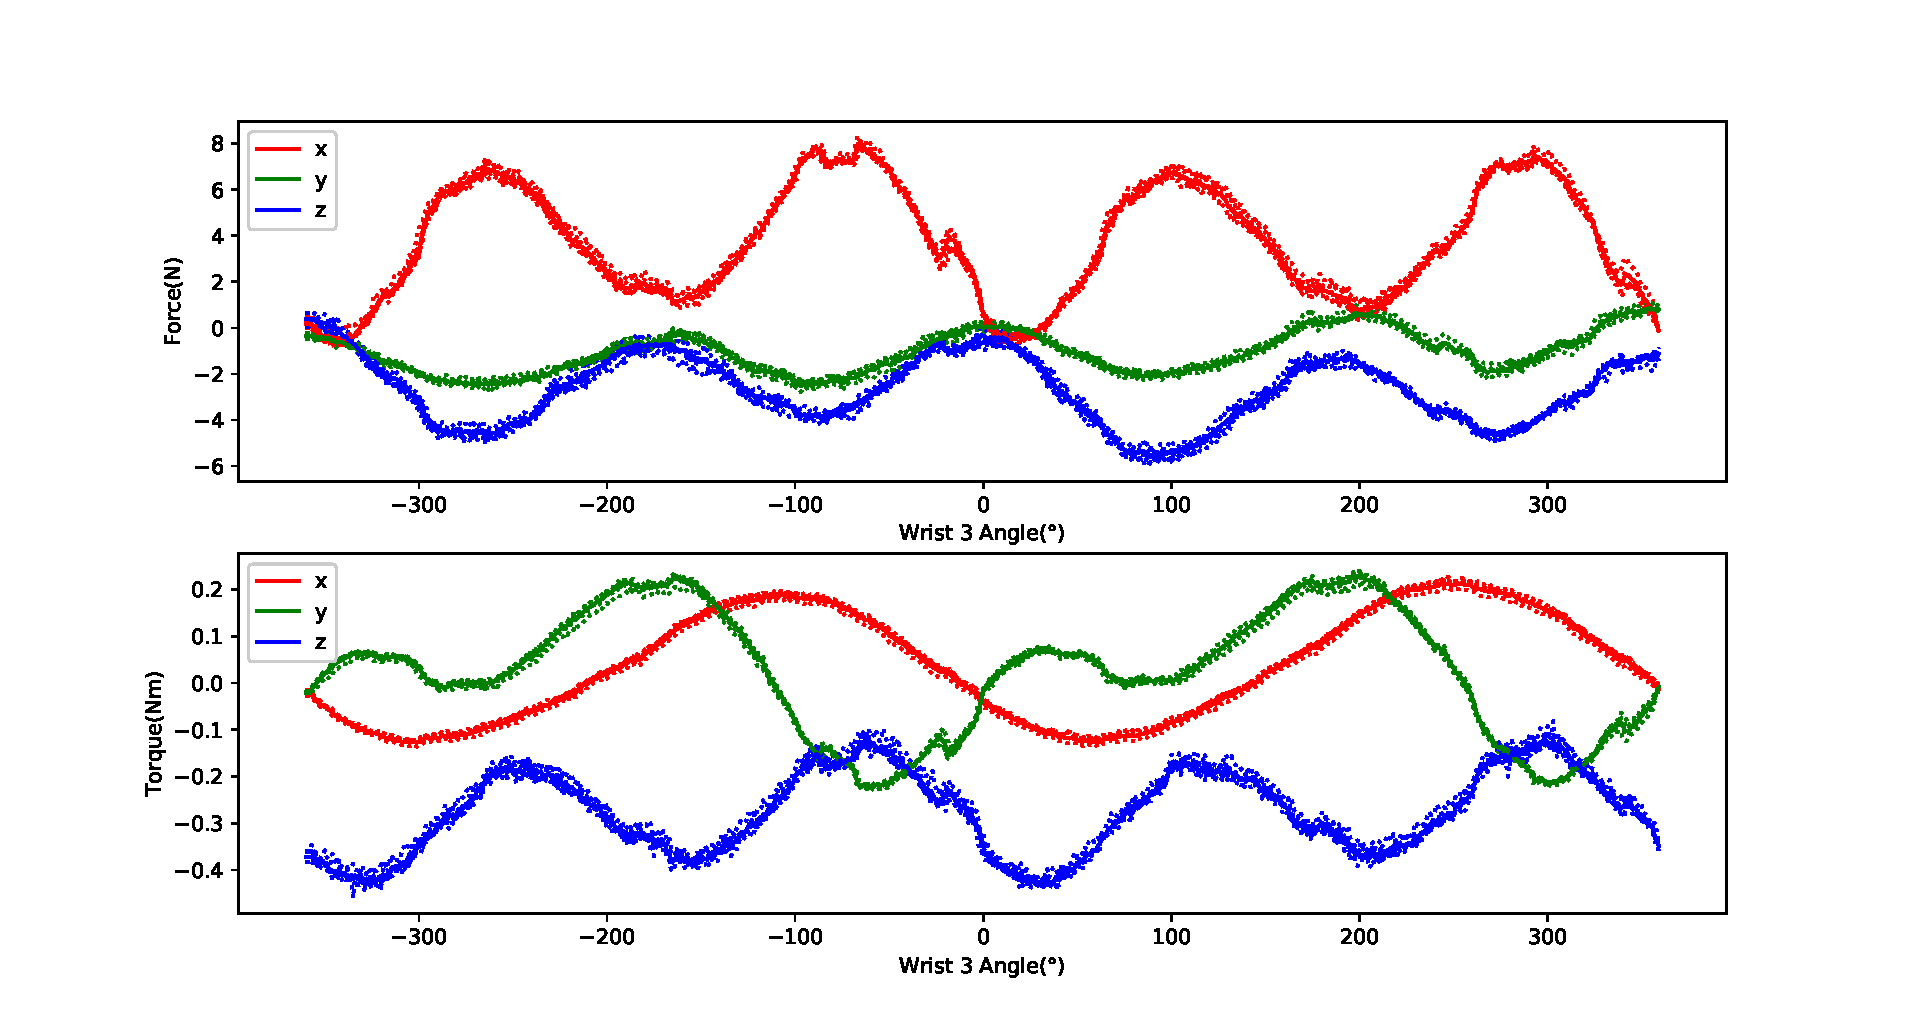
\includegraphics[width=\linewidth]{figs/chp3/ft_sensor_test_5.pdf}
    \caption{Average \ac{ft} values in the 5 testing poses}
    \label{fig:ft_sensor_test_5}
\end{figure}


\par As such, from the average results of the tests performed, a \ac{ros} node was developed to correct in real time the \ac{ft} measurements, based on the position of the Wrist3 joint. It subscribes to the filtered values of \ac{ft} from the topic \textbackslash \textit{wrench\_filtered}, and to the current position of the Wrist3 joint, present in the \textbackslash \textit{joint\_state} topic. The position of the joint serves as index to the correction matrix. The corrected values are published to the \textbackslash \textit{wrench\_corrected} topic.

\par Regarding the variations of \ac{ft} based on time and extreme contacts with the sensor, those problems become irrelevant when a cobot is placed in a real use case scenario. For the drifting problem, a simple idle mode can be implemented, where the robot is suspended if no user or program interacts with it. Once resumed, the zero\_ftsensor service can be called, making any \ac{ft} drifting measurements disappear. In the case of the variation of \ac{ft} due to external forces, the solution once again relies on the sensor taring service, since the system can be programmed to trigger it in multiple scenarios, such as a state change or the release of the gripper tool. Further detail on the use of this service, in conjunction with a global state machine to solve the inaccuracies of the \ac{ft} sensor are described in \autoref{chapter:colab-tasks}.

% Falta referir Time Series Analysis

\subsection{Results}

\par With the implementation of the correction node, the results from the real time test firstly shown in \autoref{fig:w3_problem} are satisfactory, and presented \autoref{fig:w3_result}.

\begin{figure}[h]
    \centering
    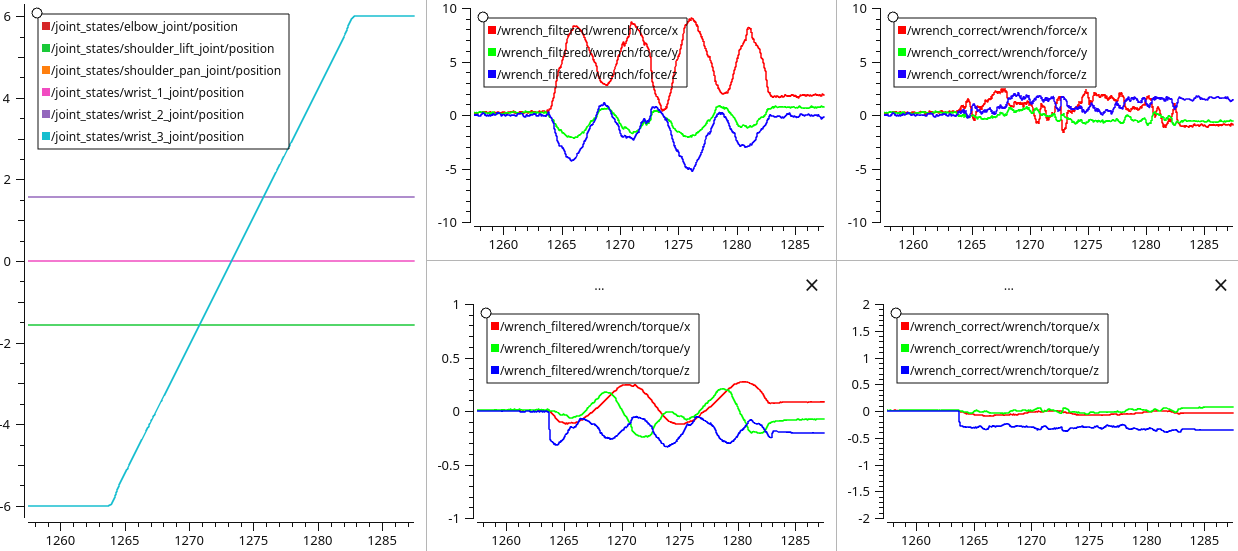
\includegraphics[width=0.9\linewidth]{figs/chp3/wrist_3_result.png}
    \caption{Result of the correction node applied in the initial test}
    \label{fig:w3_result}
\end{figure}

\par The results are as expected. Since the observed pattern is caused by the position of the Wrist3 joint, and is highly repeatable, the corrected \ac{ft} measurements present themselves relatively close to 0 since the \ac{eef} once again has nothing attached. Some variation is still present but in the case of the real time test, it is caused bu the nature of the test, since the movement of the Wrist3 joint is continuos, vibrations and jitters (\textbf{CONTINUAR})

\par Mention that the results are good , that the variation comes from the continuous movement of wrist 3 and that the real difference can be seen on the histogram


\begin{figure}[h]
    \centering
    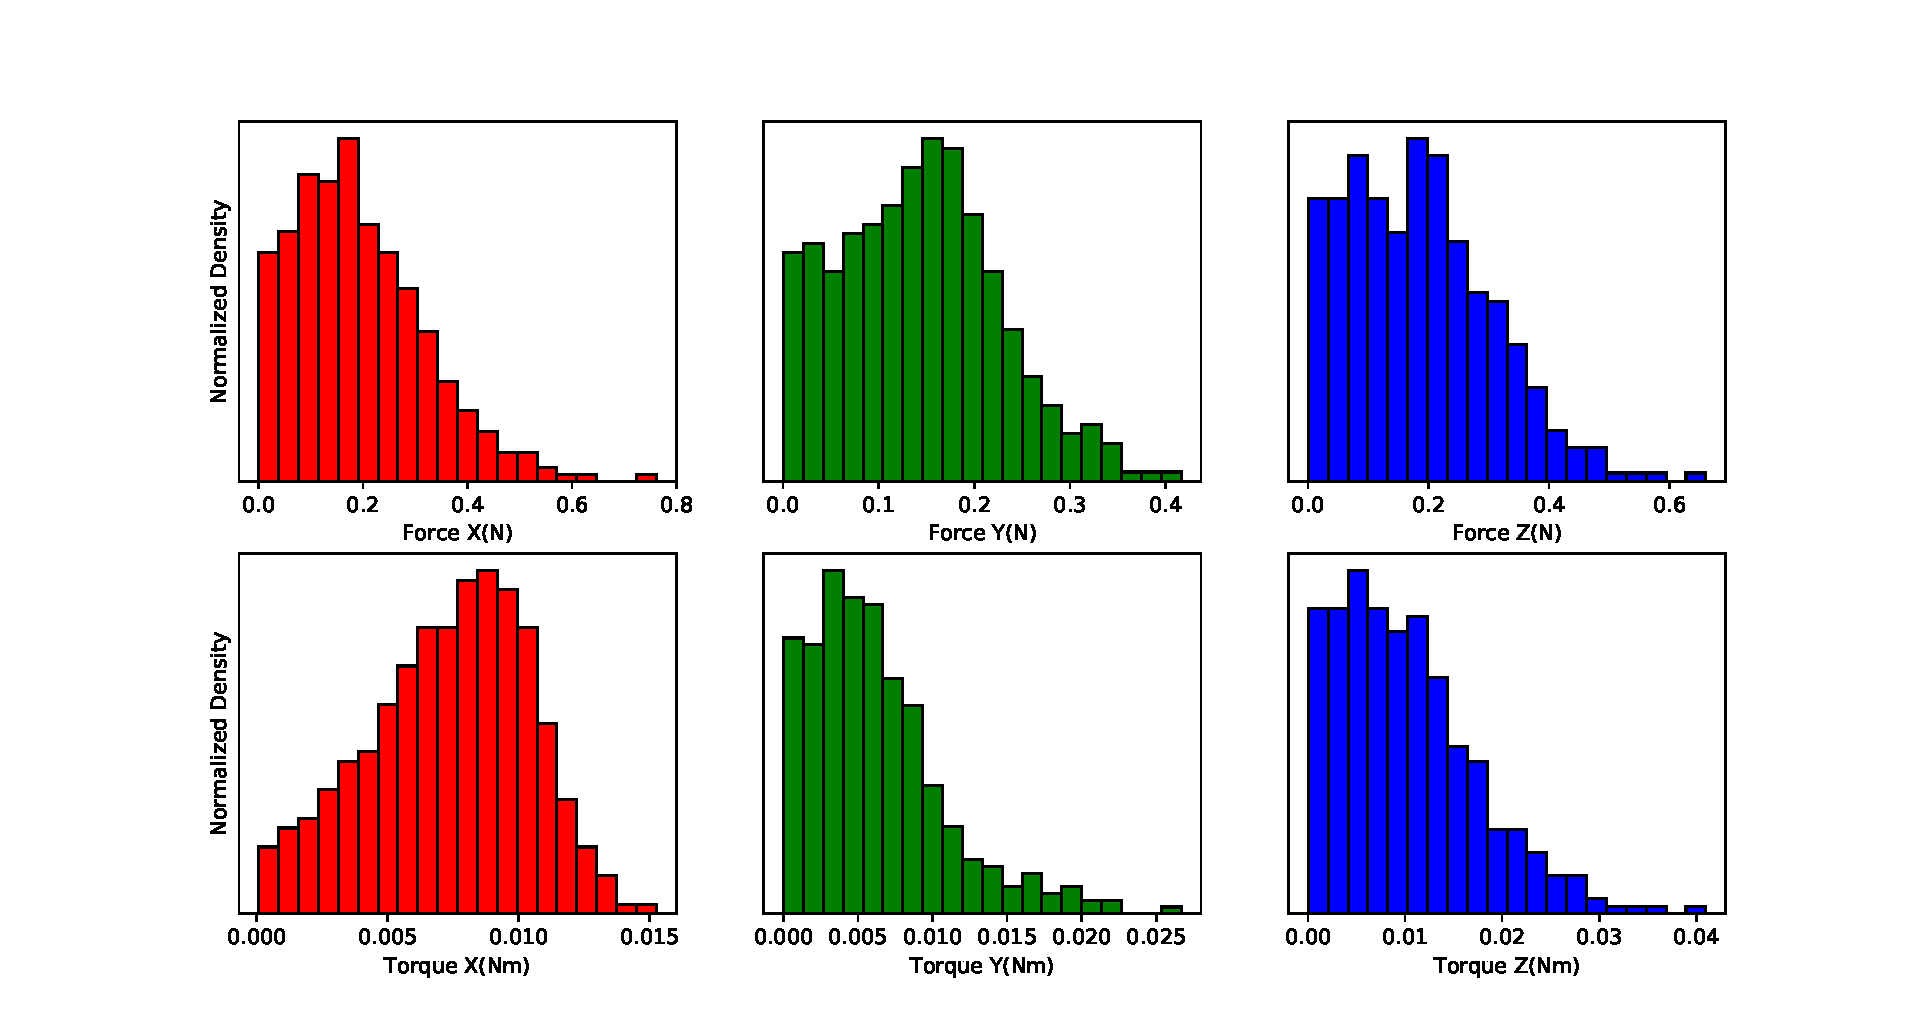
\includegraphics[width=\linewidth]{figs/chp3/wrist_3_result_hist.pdf}
    \caption{Histogram showing the difference from the correct function}
    \label{fig:w3_result_hist}
\end{figure}


\section{End Effector Weight Compensation}

\par For effective hand guide the robot with attached tools and objects, the effects of the weight and cog of the object must be compensated, so a model of the behavior of the FT sensor must be created...

\subsection{UR FT Sensor Controller Internal Compensation}
\label{ssec:ft_internal_comp}

\par The user only has access to the FT values from that are published by the controller. Furthermore if the user changes the internal payload weight and center of gravity parameters, the controller behavior will change

\par Behavior of the sensor with Payload configured to 1.5Kg and Cog [0, 0, 100] and nothing attached to the EEF

\begin{figure}[h]
    \centering
    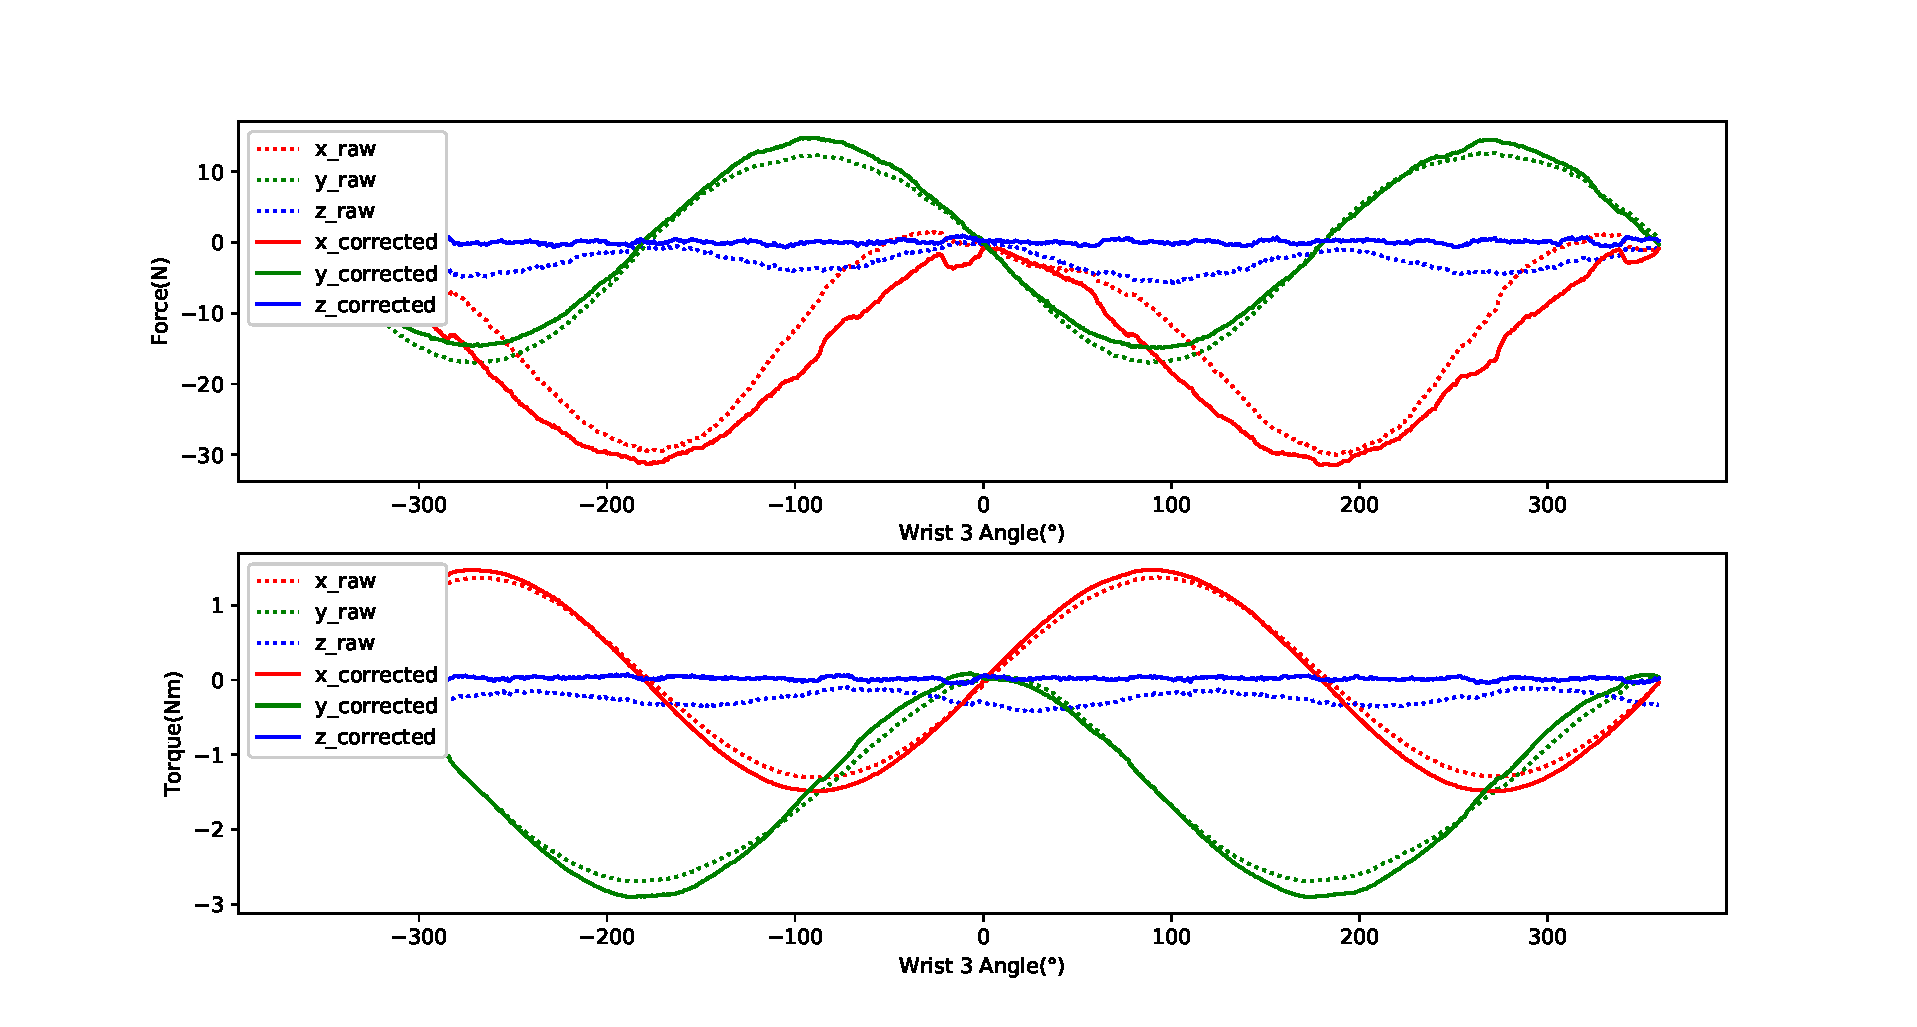
\includegraphics[width=\linewidth]{figs/chp3/ft_sensor_behavior.pdf}
    \caption{Behavior of the FT sensor with parametrization of payload and cog }
    \label{fig:ft_sensor_behavior}
\end{figure}

\par This means that the behavior of the ft sensor changes depending on the configured payload and cog and because there is no knowledge on the implementation of hte controller, the values that will be considered from here forward are payload 0 and cog 0 to get a consistent behavior independent of the weight of hte object 


\subsection{FT Theoretical Model}

\par Based on the knowledge of the weight and cog of the attached object this model should give the theoretical values that a FT sensor should have

\subsubsection{Force}

\par Explain the force generation model

\begin{figure}[h]
    \centering
    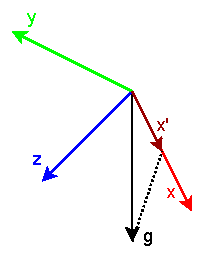
\includegraphics[width=0.3\linewidth]{figs/chp3/ft_theory_force.pdf}
    \caption{Visualization of generation of theoretical force values}
    \label{fig:ft_theory_force}
\end{figure}

\[ Fx = \langle \hat{x_{eef}} , \hat{g} \rangle \cdot m \cdot g \]

\subsubsection{Torque}

\par Explain the torque generation model

\begin{figure}[h]
    \centering
    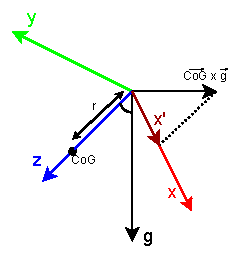
\includegraphics[width=0.35\linewidth]{figs/chp3/ft_theory_torque.pdf}
    \caption{Visualization of generation of theoretical torque values}
    \label{fig:ft_theory_torque}
\end{figure}

\[ Tx = \langle\hat{x_{eef}} , \vec{CoG} \times \vec{g} \rangle \cdot m \cdot g\cdot r \]

% O melhoramento desta função tem a haver com a seguinte divisao
% para a obtenção de um torque em X, ha 3 componentes
%     1 - mg -> sempre
%     2 - que tem a haver com a rotação em Y -> r.sin(theta)
%     3 - que tem a haver com a rotação em Z -> < X , cog x g>
% Tabem pode ser possivel alterar esta equacao para
%     1 - mg -> sempre
%     2 - que tem a haver com a rotacao em Y -> r(vetor com 3 comp) x sin(angulo que faz com o eixo)
%     3 - que tem a haver com a rotação em Z -> projecção do vetor g no plano cujo vetor normal é o eixo

\subsection{Results}

\par With a configured weight of 1.5Kg, Cog (0, 0, 0.45) and with an EEF orientation of (specify orientation)

\par below is a comparison of the values from the sensor (corrected) and the theory model

\begin{figure}[h]
    \centering
    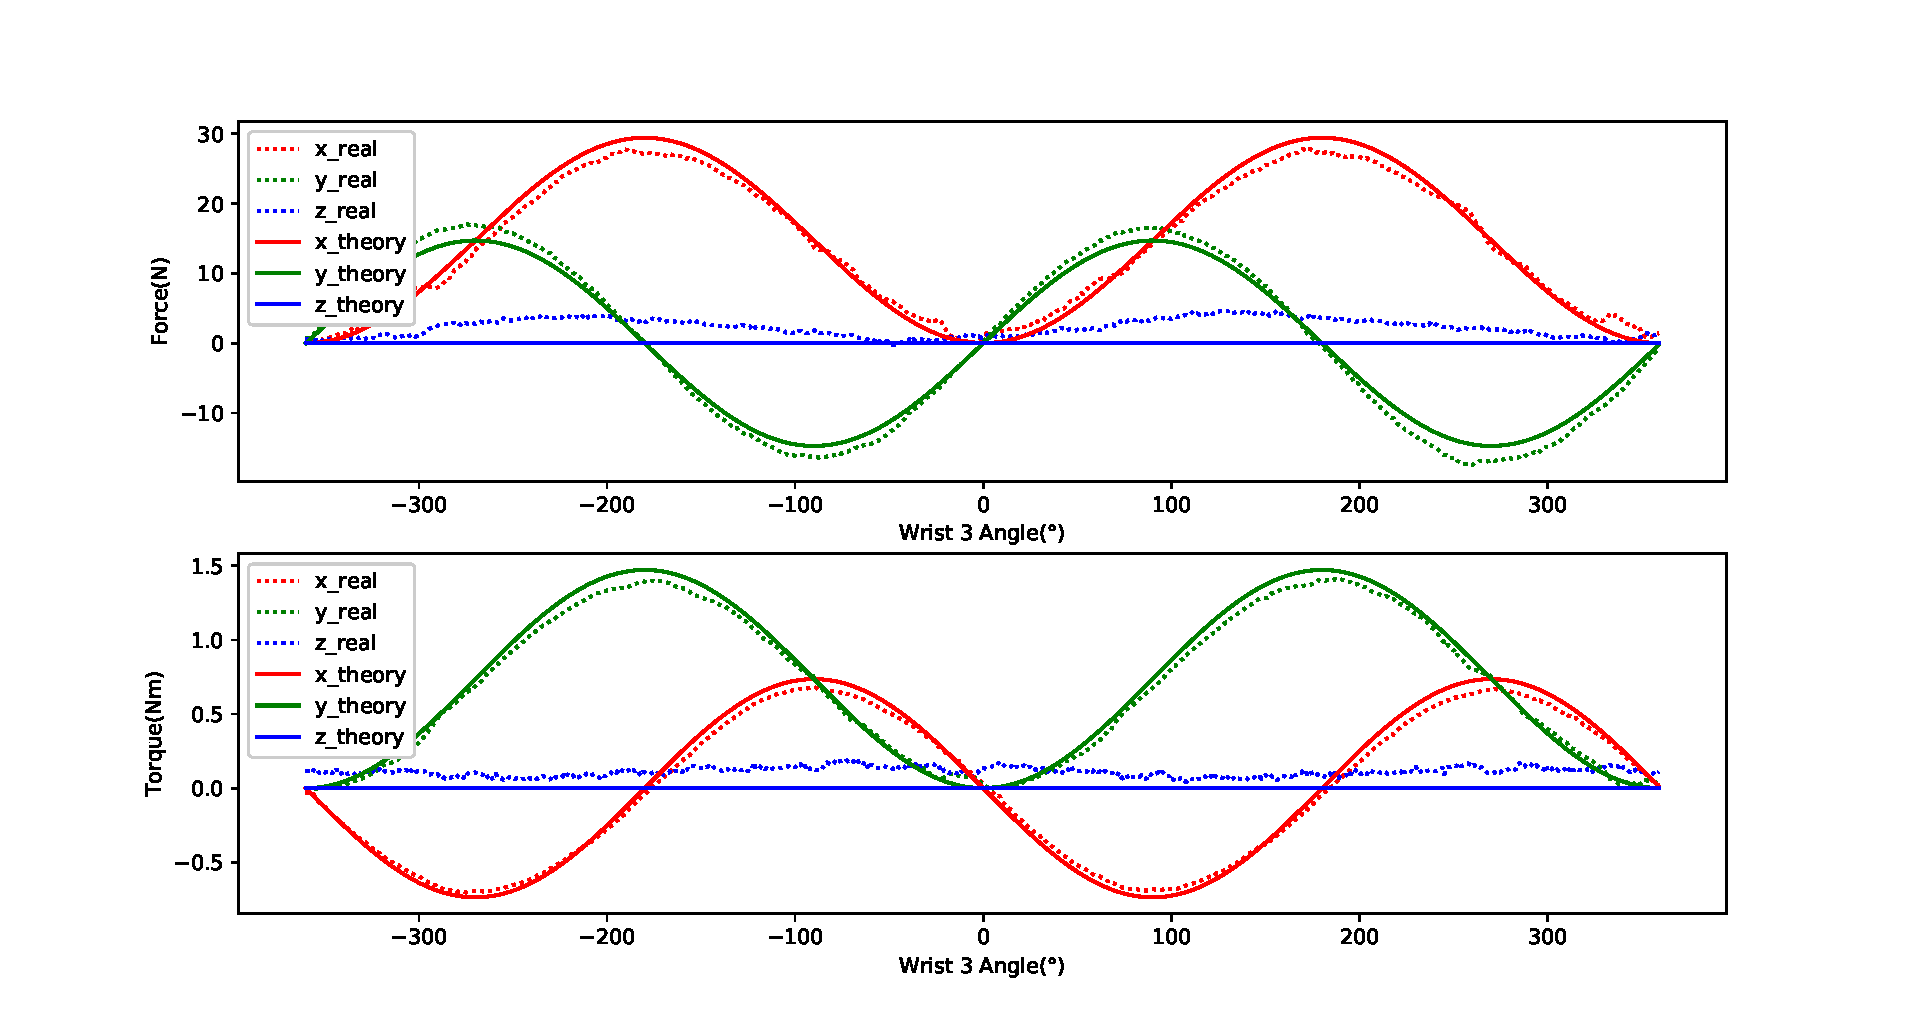
\includegraphics[width=\linewidth]{figs/chp3/ft_sensor_theory.pdf}
    \caption{Visualization of generation of theoretical torque values}
    \label{fig:ft_sensor_theory}
\end{figure}



\par Below is an histogram for a better understanding of the distribution of the erros between the 2 things

\begin{figure}[h]
    \centering
    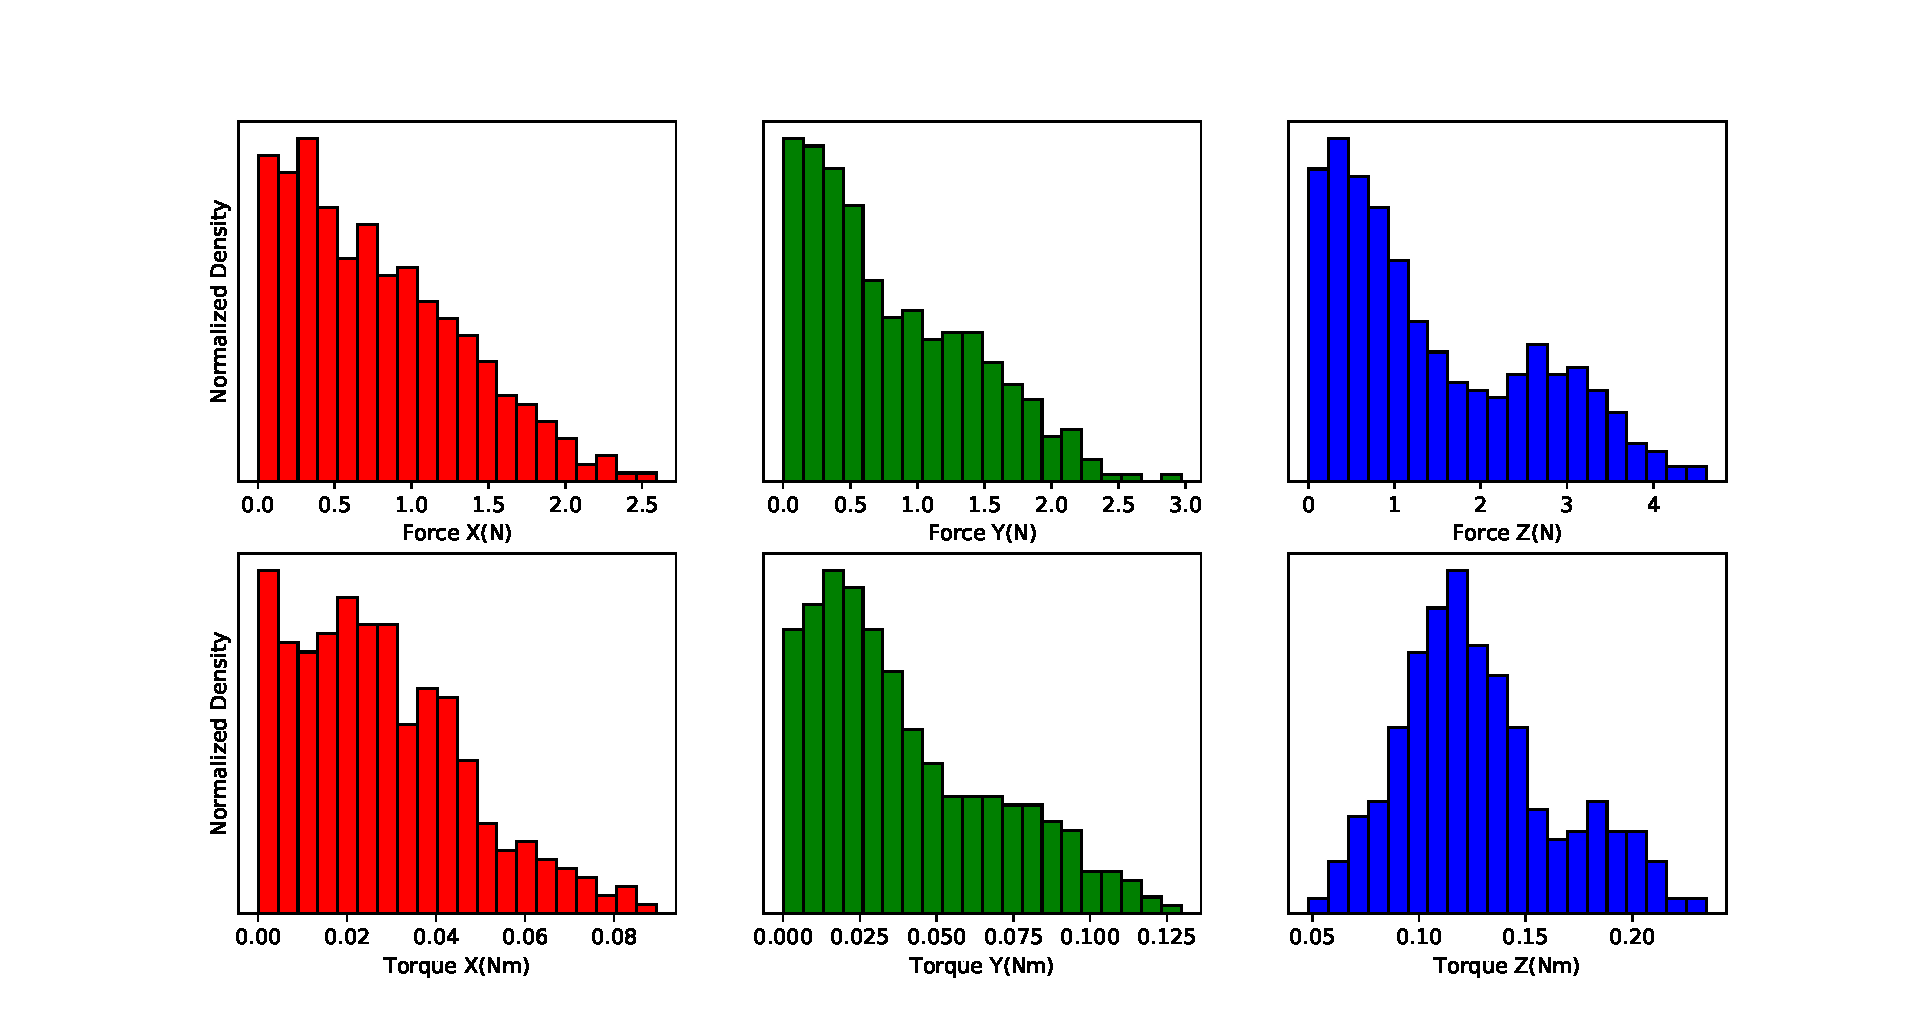
\includegraphics[width=\linewidth]{figs/chp3/ft_sensor_theory_hist.pdf}
    \caption{Visualization of the difference of the 2 things}
    \label{fig:ft_sensor_theory_hist}
\end{figure}

\par There is still some difference


\subsection{Correction of the FT Model based on Observations}

\par so aqui é que se fala das 57 posições e mais nao sei que

\begin{figure}[h]
    \centering
    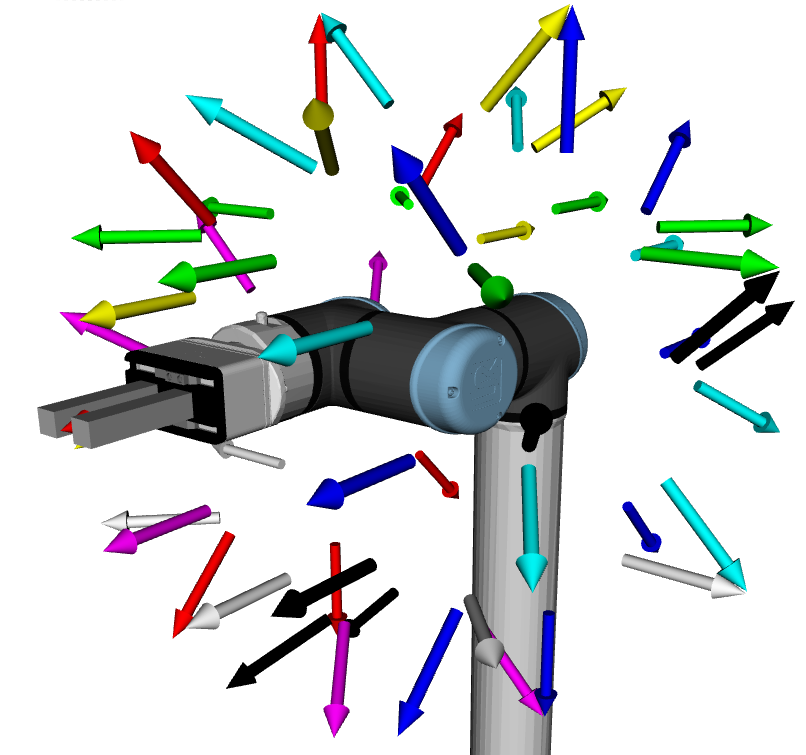
\includegraphics[width=0.35\linewidth]{figs/chp3/globe_57.png}
    \caption{Visualization of the 57 poses in which the tests were performed}
    \label{fig:57_poses}
\end{figure}

\par in each position a regular test was made and the result saved. then an optimization function was performed for each of them 

\par after inputing in the theoreticl model the results from the optimization function, the results obtained are as follow

% correr a função de otimização

\begin{figure}[h]
    \centering
    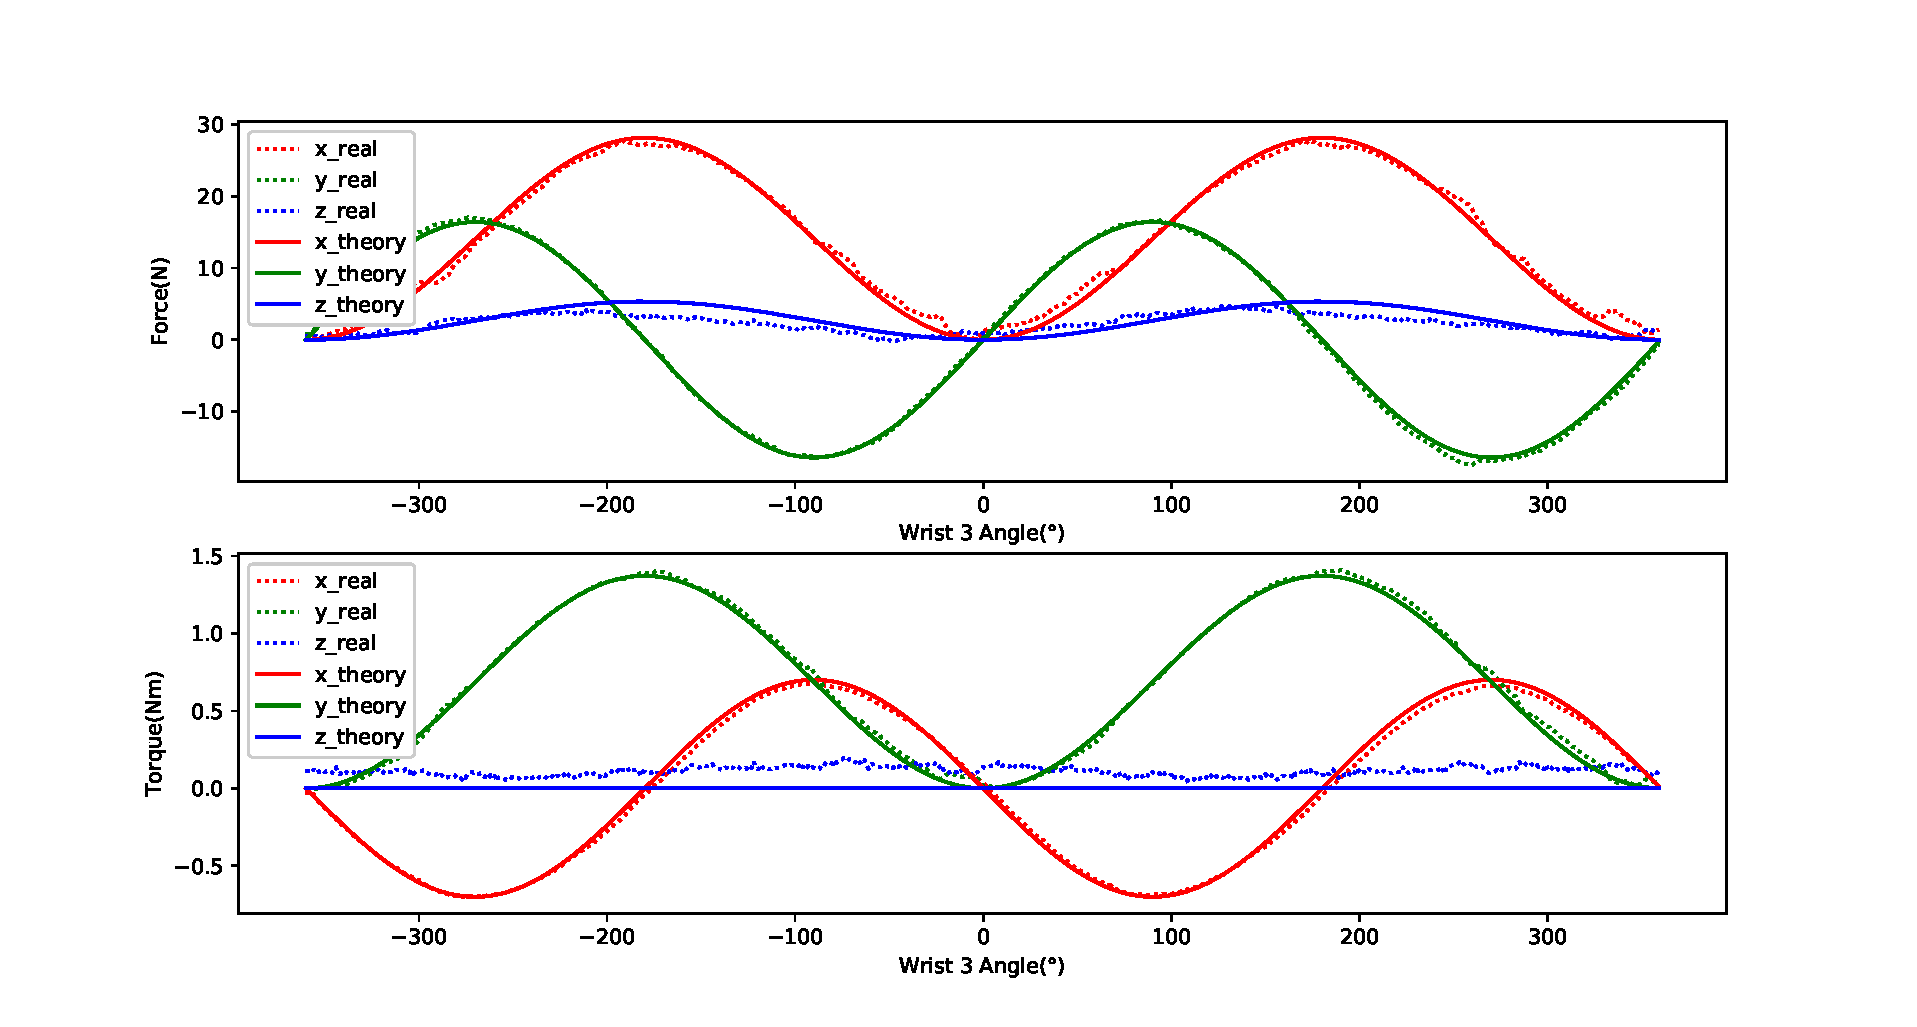
\includegraphics[width=\linewidth]{figs/chp3/ft_sensor_theory_adjust.pdf}
    \caption{Visualization of generation of theoretical torque values adjusted}
    \label{fig:ft_sensor_theory_adjust}
\end{figure}

\begin{figure}[h]
    \centering
    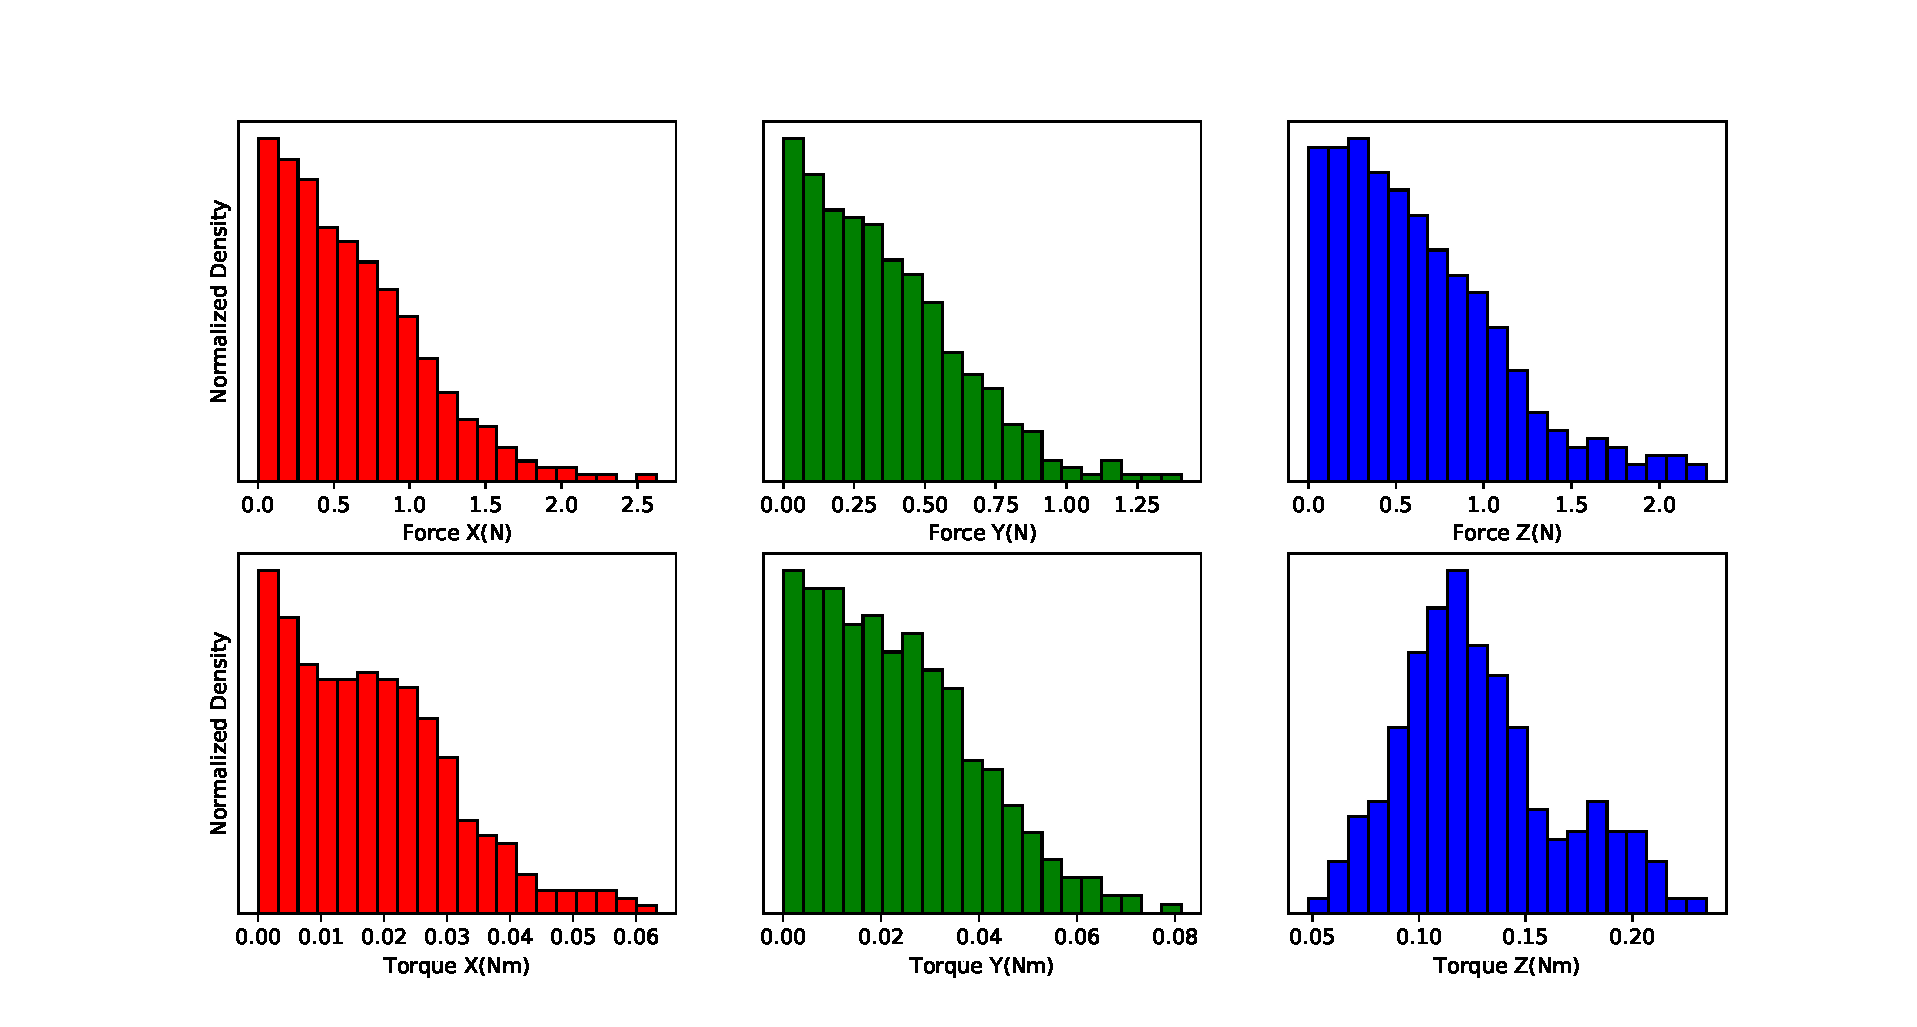
\includegraphics[width=\linewidth]{figs/chp3/ft_sensor_theory_adjust_hist.pdf}
    \caption{Visualization of the difference of the 2 things adjusted}
    \label{fig:ft_sensor_theory_adjust_hist}
\end{figure}

\subsection{Real Time Correction and Compensation of \ac{ft}}

\begin{figure}[h]
    \centering
    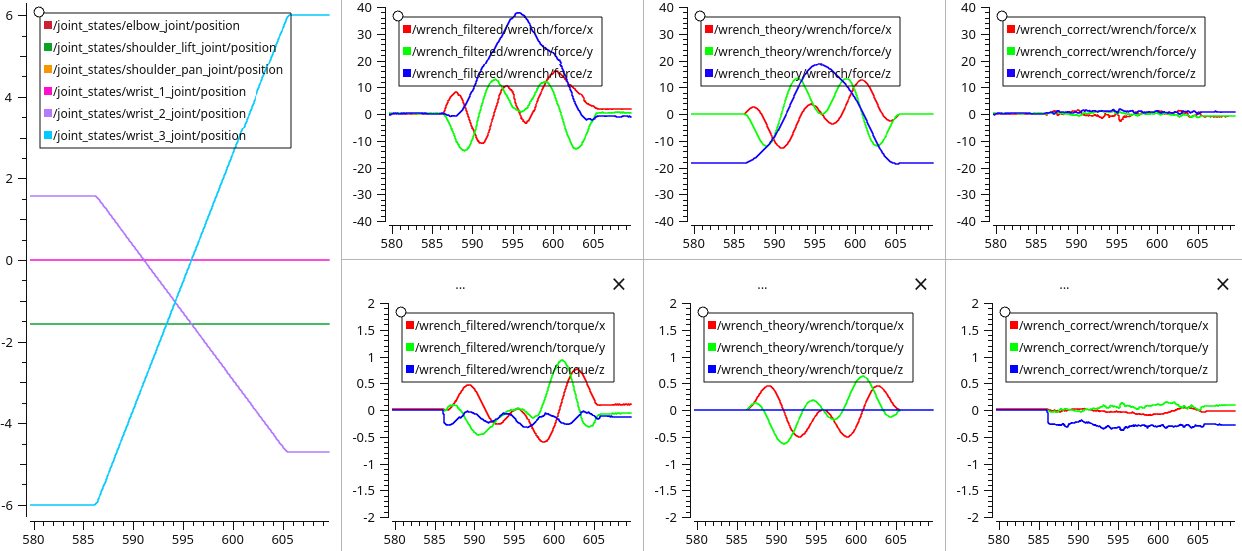
\includegraphics[width=0.9\linewidth]{figs/chp3/ft_sensor_theory_result.png}
    \caption{Result of the compensation node applied in the initial test}
    \label{fig:ft_theory_result}
\end{figure}
